\documentclass[final]{beamer}

% ====================
% Packages
% ====================

\usepackage[T1]{fontenc}
\usepackage{lmodern}
\usepackage{amsmath}
\usepackage[size=a0,scale=1.25,orientation=portrait]{beamerposter}
\usepackage[backend=biber,style=apa,citestyle=apa,doi=false,isbn=false,url=false,eprint=false]{biblatex}
\addbibresource{poster.bib}
\usetheme{gemini}
\usecolortheme{unisg}
\usepackage{graphicx}
\usepackage{booktabs}
\usepackage{tikz}
\usepackage{xcolor} % Link / Citation colors
\usepackage{hyperref} % HRef / Citations
\usepackage{anyfontsize}
\usepackage{colortbl}

\newcommand\myshade{85}
\colorlet{mylinkcolor}{unisgdarkgreen}
\colorlet{mycitecolor}{unisgdarkgreen}
\colorlet{myurlcolor}{unisgdarkgreen}
\urlstyle{rm}
\hypersetup{
	linkcolor  = mylinkcolor!\myshade!black,
	citecolor  = mycitecolor!\myshade!black,
	urlcolor   = myurlcolor!\myshade!black,
	colorlinks = true,
}

% ====================
% Lengths
% ====================

% If you have N columns, choose \sepwidth and \colwidth such that
% (N+1)*\sepwidth + N*\colwidth = \paperwidth
\newlength{\sepwidth}
\newlength{\colwidth}
\newlength{\colwidthsmall}
\newlength{\colwidthlarge}
\setlength{\sepwidth}{0.02\paperwidth}
\setlength{\colwidth}{0.47\paperwidth}
\setlength{\colwidthsmall}{0.34\paperwidth}
\setlength{\colwidthlarge}{0.6\paperwidth}

\newcommand{\separatorcolumn}{\begin{column}{\sepwidth}\end{column}}

% ====================
% Title
% ====================

\title{Constructing Efficient Simulated Moments Using Temporal Convolutional Networks}

\author{Jonathan Chassot \inst{1} \and Michael Creel \inst{2}}

\institute[shortinst]{\inst{1} Faculty of Mathematics and Statistics, University of St.Gallen, Switzerland \\ \inst{2} Universitat Autònoma de Barcelona, Barcelona School of Economics, and MOVE, Bellaterra (Barcelona), Spain}

% ====================
% Footer (optional)
% ====================

\footercontent{
  % jonathan.chassot@unisg.ch \hfill
  34\textsuperscript{th} (EC)\textsuperscript{2} conference on Identification and Inference in Structural Econometric Models, December 8-9, 2023 \hfill
  jonathan.chassot@unisg.ch
  }
% (can be left out to remove footer)

% ====================
% Logo (optional)
% ====================

% use this to include logos on the left and/or right side of the header:
\logoleft{
\includegraphics[height=7cm]{img/HSG_Logo_White.pdf}}
\logoright{\includegraphics[height=7cm]{img/qrcode.eps}}

% ====================
% Body
% ====================


\begin{document}


\begin{frame}[t]
    \begin{columns}[t]
    \separatorcolumn
    
    \begin{column}{\colwidthsmall}
      \begin{block}{Motivation}
      \heading{Accurately modeling complex economic phenomena often presents statistical challenges, especially when traditional models lack tractable likelihoods or theoretical moments.}
      Simulation-based inference methods such as the Simulated Method of Moments \parencite[SMM;][]{McFadden1989}, Approximate Bayesian Computation \parencite[ABC;][]{Rubin1984}, or Indirect Inference \parencite[II;][]{Gourieroux1993} offer effective solutions for these challenges. These approaches involve comparing actual data with simulated data, employing moment conditions, summary statistics, or auxiliary models to evaluate the resemblance between the datasets.
      \heading{The efficacy of simulation-based inference hinges on selecting appropriate moment conditions or summary statistics.}
      Choosing the optimal moment conditions is daunting. It requires a researcher's insight into the specific problem and a careful balance between efficiency and complexity. Although overidentification doesn't compromise an estimator's consistency, it can lead to increased bias and variance in limited samples \parencite{Donald2009}.
      \heading{We alleviate the researcher's burden by learning the optimal moment conditions using deep neural networks.}
      This approach lets the data unveil its own narrative, unbiased from the researcher's assumptions. If the network is able to accurately identify the parameters of the data generating process, the output is informative and provides an exactly identifying set of statistics which can serve to construct moment conditions or summary statistics. We show by empirical example that this approach can lead to efficient estimators that rival the performance of the maximum likelihood estimator (MLE) in moderately-sized samples.    
      \end{block}
    
      \begin{alertblock}{Our Contribution}
        We introduce a novel data-driven method for creating optimal moment conditions tailored for simulation-based inference techniques. This approach involves training deep neural networks on simulated data to pinpoint parameters of the data-generating process (DGP).

        \heading{Construction vs. Selection}
        Unlike most existing literature which primarily focuses on selecting moment conditions from a predetermined set, our method removes this requirement by leveraging the networks' ability to model complex non-linear relationships, enabling the construction of moment conditions directly from the DGP.

        \heading{Harnessing the Power of Simulations}
        We exploit the simulable nature of the DGP by training the networks on an arbitrarily large number of simulated data points. Allowing us to circumvent the typical data scarcity issues that plague deep learning applications.

        \heading{Avoiding Overidentification}
        The output from our networks is designed to be exactly identifying, providing unique statistics that precisely determine the DGP parameters, thereby bypassing the overidentification issues often encountered in finite sample scenarios.
        
        \heading{Beyond Point Estimation}
        While neural networks excel in parameter estimation, they fall short in providing measures of statistical uncertainty. Our approach, in conjunction with methods like SMM, ABC, or II, complements the network's estimations with a robust framework for inference, utilizing the network's output solely as an intermediate step.         
      \end{alertblock}
    \end{column}
    
    \separatorcolumn
    
   
    \begin{column}{\colwidthlarge}

      \begin{block}{Empirical Examples}
        \begin{enumerate}
          \item We assess our estimator's performance against the MLE using three straightforward DGPs with tractable likelihoods: MA(2), Logit, and GARCH(1, 1) models.
          \item Our method is further tested on a jump-diffusion stochastic volatility model applied to S\&P 500 returns, where we benchmark our estimator against an approach using traditional moment conditions.
        \end{enumerate}
      \end{block}\vspace{-.5em}

      \begin{block}{MA(2), Logit, GARCH(1, 1)}    
        \begin{figure}
          \centering
          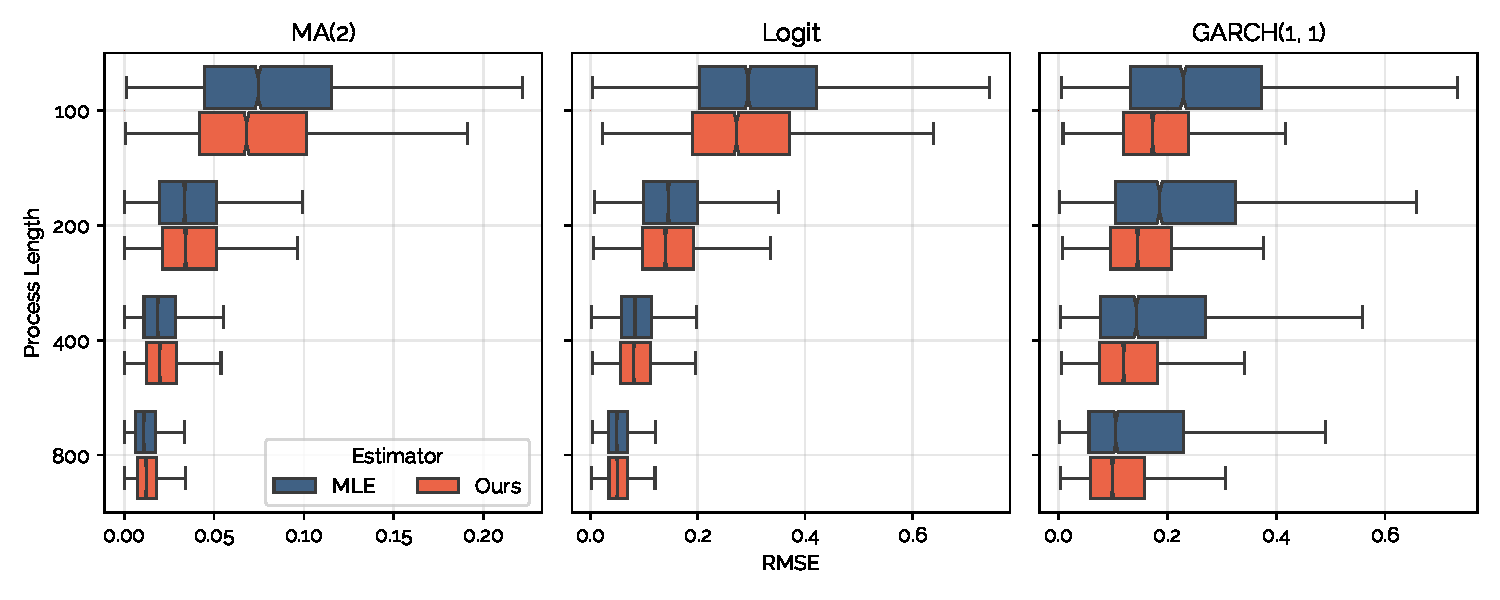
\includegraphics[width=\textwidth]{img/errors.pdf}
          \caption{Boxplots of the average root mean squared error (RMSE) of the point estimates of each parameter for the three models with tractable likelihoods.}
        \end{figure}      
      \end{block}\vspace{-.5em}

      \begin{block}{Jump-Diffusion Stochastic Volatility}

      \begin{table}
        \begin{tabular}{lrrrrrrrr}
          \toprule
          {} & \multicolumn{8}{c}{\text{Parameter}}\\
          \cmidrule(lr){2-9}
          \textbf{Bias} &  $\mu$ &  $\kappa$ &  $\alpha$ &  $\sigma$ &  $\rho$ & $\lambda_0$ & $\lambda_1$ &  $\tau$ \\
          \midrule
          \textit{Standard} Moments & 0.003 & \textbf{0.001} & -0.072 & 0.021 & -0.008 & 0.004 &0.325 & 0.000 \\
          Our Method  &  \textbf{-0.002} & 0.005 & \textbf{0.023} & \textbf{0.005} & \textbf{0.006} & \textbf{0.002} & \textbf{0.065} & \textbf{0.000}\\
          \arrayrulecolor{white}
          \midrule
          \textbf{RMSE} &  $\mu$ &  $\kappa$ &  $\alpha$ &  $\sigma$ &  $\rho$ & $\lambda_0$ & $\lambda_1$ &  $\tau$ \\
          \arrayrulecolor{black}
          \midrule
          \textit{Standard} Moments & 0.015 & 0.021 & 0.212 & 0.077 & 0.047 & 0.006 & 0.800 & 0.001\\
          Our Method  &  \textbf{0.011} & \textbf{0.018} & \textbf{0.142} & \textbf{0.057} & \textbf{0.032} & \textbf{0.005} & \textbf{0.636} & \textbf{0.001}\\
          \bottomrule
        \end{tabular}
        \caption{Average bias and RMSE of the estimates from simulation-based inference using our method and \textit{standard} moments (means, standard deviations, first-order autocorrelations, and correlations across variable pairs of price, realized volatility, and bipower variation). 100 replications}
        \label{tab:results}
      \end{table}

      \begin{figure}\label{fig:results}
        \centering
        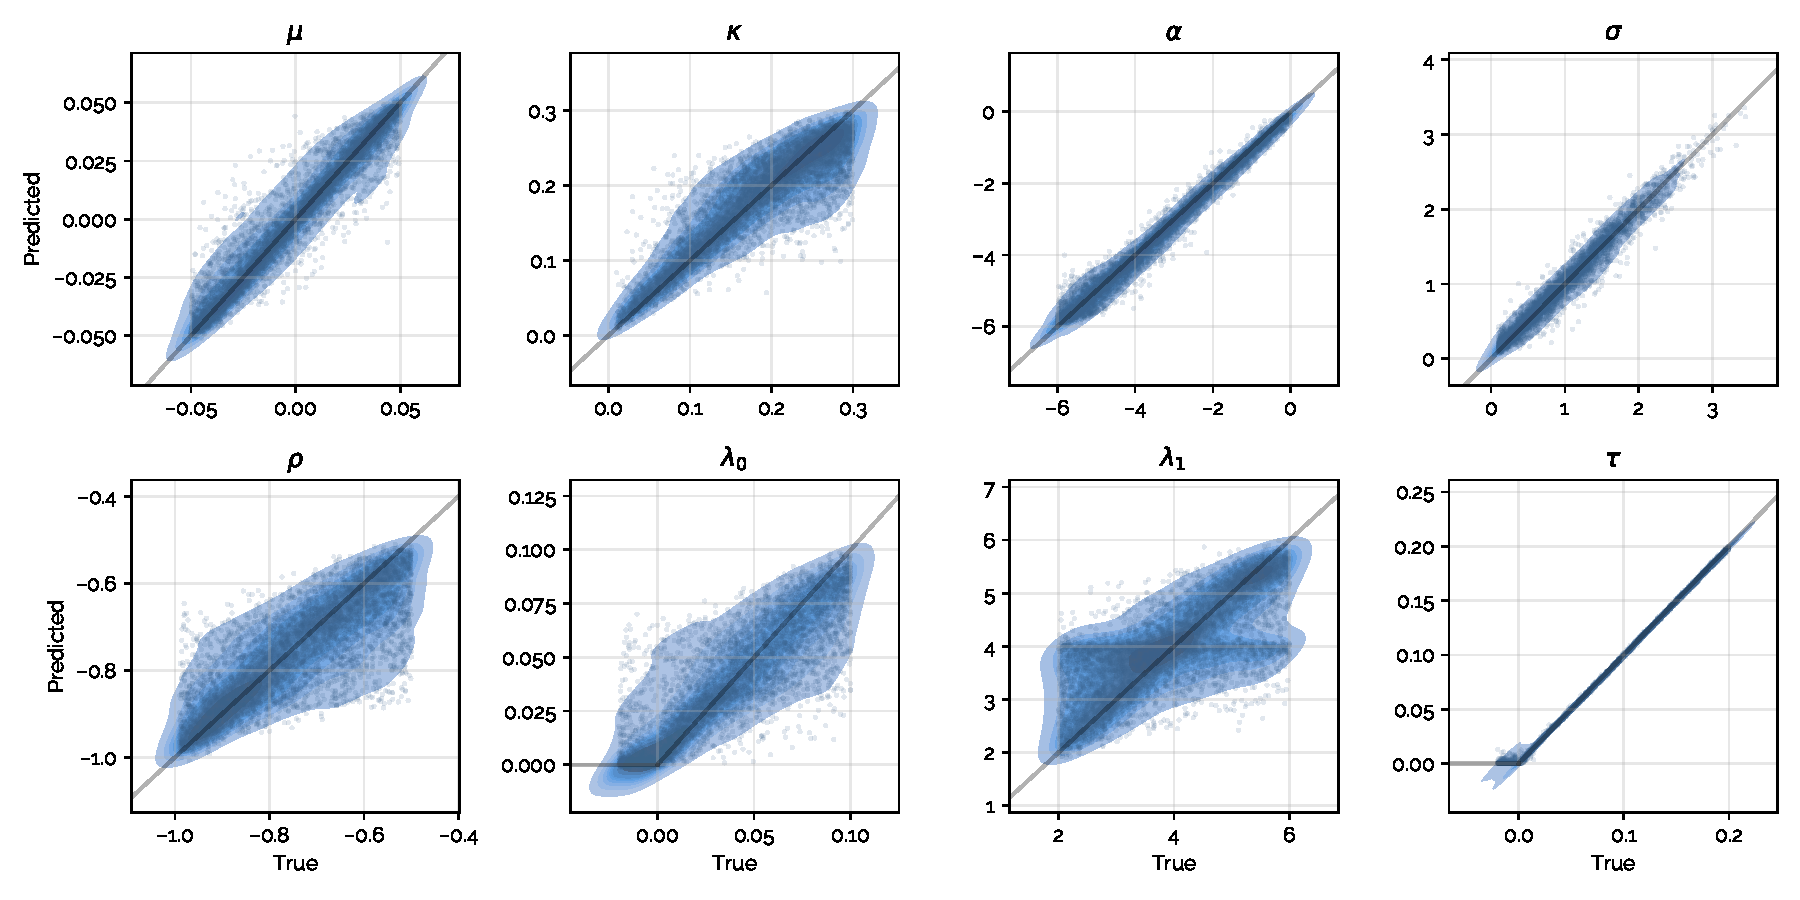
\includegraphics[width=\textwidth]{img/preds_poster.pdf}\vspace{-1em}
        \caption{True values against predicted values for the jump-diffusion model parameters. 5\,000 replications.}
      \end{figure}  

      \end{block}\vspace{-1em}

    
      \begin{block}{References}
        \printbibliography
      \end{block}
    

      
      

      
    \end{column}
    
    \separatorcolumn
    
    \begin{column}{\colwidth}
      
    \end{column}
    
    \separatorcolumn
    \end{columns}
    \end{frame}
\end{document}
